\chapter{Linda}

\section{Il Modello Linda}

\subsection{Introduzione}

\paragraph{Nei linguaggi tipo Ada o nel linguaggio dei transputer, i processi comunicano mediante un meccanismo sincrono:}

\begin{itemize}
	\item Connessi nel tempo: sincronia.
	\item Connessi nello spazio: indirizzo del canale.
\end{itemize}

\paragraph{Linda permette:}

\begin{itemize}
	\item Il \fancyglitter{disaccorpamento} nel tempo e nello spazio.
	\item La \fancyglitter{persistenza dell'informazione} per cui i dati (messaggi) possono esistere anche dopo la terminazione del processo che li ha creati.
\end{itemize}

\dfn{Linda}{
	Il modello Linda definisce una struttura globale detto spazio delle tuple
	che si può immaginare come una grande bacheca su cui si possono
	attaccare dei post-it, chiamati note o tuple.
}

\cor{Tupla}{
	Una tupla è una sequenza tipata di dati.
}

\paragraph{Il match di due tuple si verifica se hanno lo stesso numero di valori e se i
	valori nelle medesime posizioni:}

\begin{itemize}
	\item O sono entrambi uguali, nel caso siano entrambi valori.
	\item Oppure uno è un valore e l’altro è una variabile dello stesso tipo del
	      valore.
\end{itemize}

\begin{center}
	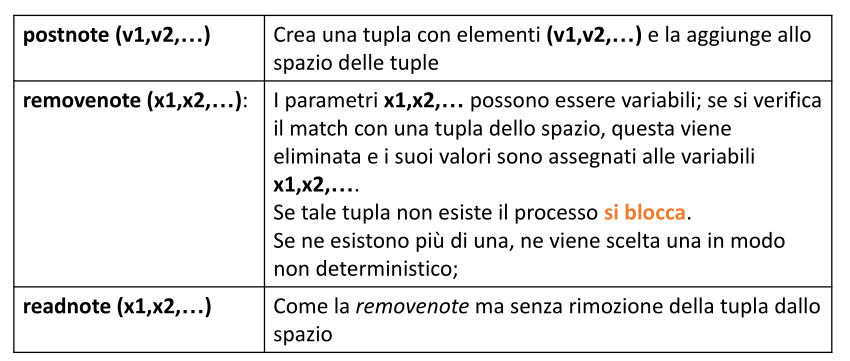
\includegraphics[scale=0.4]{06-LINDA/st.png}
\end{center}

\nt{
	Quindi le tuple di Linda possono contenere delle variabili e dei valori.
	In maniera analoga alla chiamata di procedura, il match di due tuple
	corrispondenti provoca il trasferimento dei valori attuali di una tupla
	nelle variabili dell’altra.
}

\begin{center}
	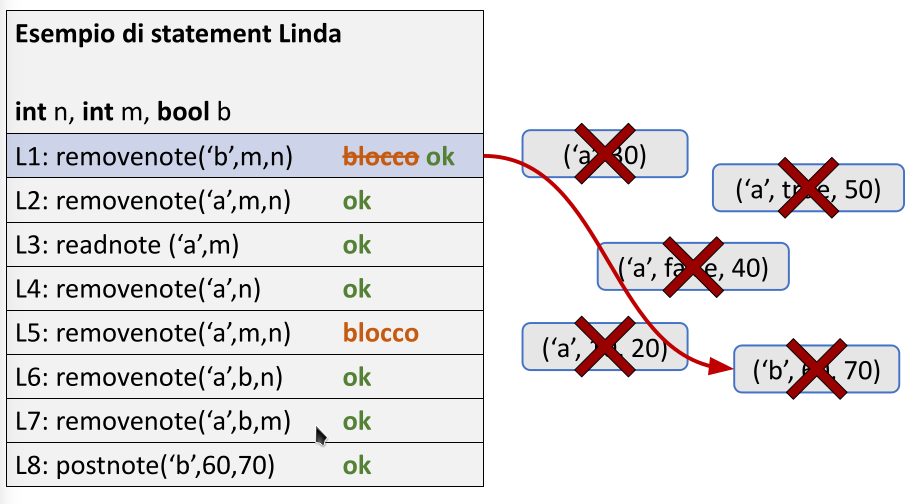
\includegraphics[scale=0.4]{06-LINDA/est.png}
\end{center}

\subsection{Rendez-vous}

\paragraph{In linda è possibile implementare il Rendez-vous, le tuple avranno come parametri:}

\begin{itemize}
	\item Stringa contente il \fancyglitter{nome del servizio}.
	\item Nome del \fancyglitter{processo chiamante}.
	\item Due \fancyglitter{parametri di input} (intero e carattere) e uno di \fancyglitter{output}.
\end{itemize}

\section{Il Paradigma Master/Workers}

\paragraph{In Linda è possibile scrivere programmi flessibili in grado di adattarsi al numero di
	processi esistenti (load balancing) utilizzando il paradigma master/workers:}
\begin{itemize}
	\item \fancyglitter{Master:} inserisce nello spazio tanti postnote quanti sono i tasks da eseguire.
	\item \fancyglitter{Worker:} recupera uno dei postnote ed esegue la computazione.
\end{itemize}

\begin{center}
	\begin{minipage}{0.45\textwidth}
		\centering
		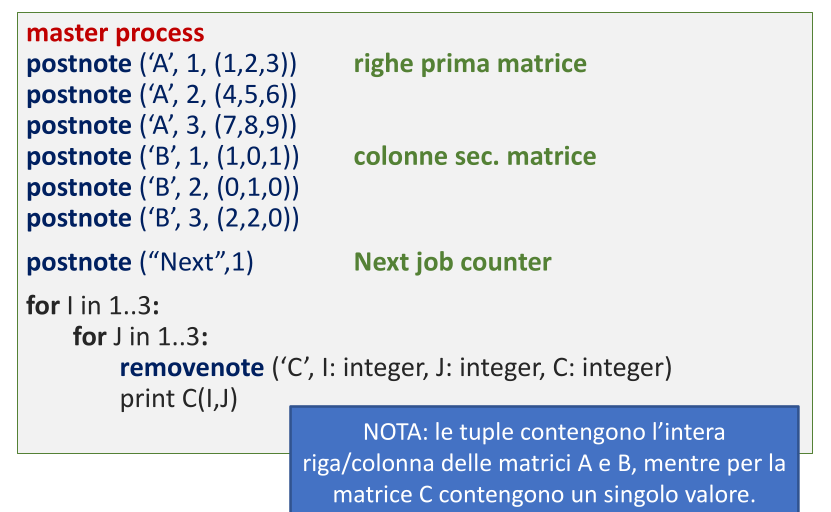
\includegraphics[scale=0.27]{06-LINDA/mmatrix.png}
	\end{minipage}
	\hfill
	\begin{minipage}{0.45\textwidth}
		\centering
		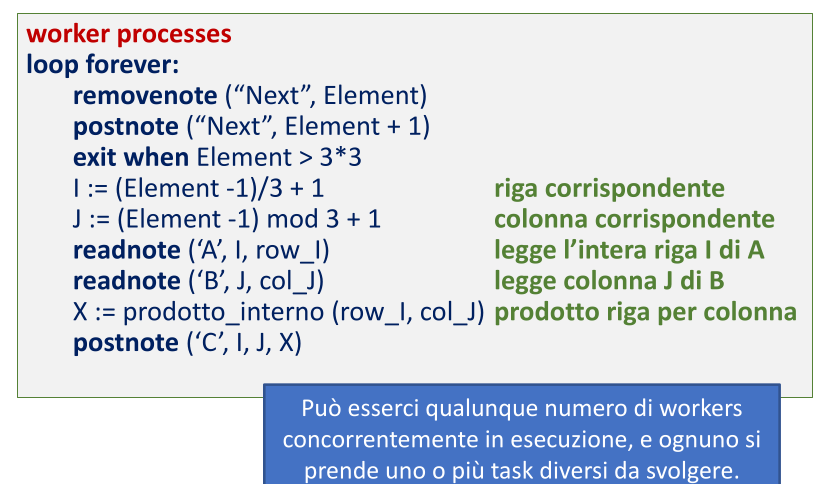
\includegraphics[scale=0.27]{06-LINDA/wmatrix.png}
	\end{minipage}
\end{center}

